\documentclass[11pt]{article}

\usepackage[margin=1.15in]{geometry}
\usepackage{amsmath,amssymb}
\usepackage{booktabs}
\usepackage{graphicx}
\usepackage{caption}
\usepackage{microtype}
\usepackage[hidelinks]{hyperref}
\usepackage{siunitx}
\usepackage{enumitem}

\sisetup{detect-all, table-format=+1.4, group-digits=false}
\captionsetup{font=small, labelfont=bf, skip=8pt}
\setlist{itemsep=2pt, topsep=4pt}

\newcommand{\fac}[1]{\texttt{\small #1}}

\title{\bfseries Two Bugs, Two Fingerprints:\\[2pt]
Identifying Data-Handling Errors from the\\Cross-Section of Reported Factor Performance}

\author{Raunak Sood\\
\normalsize University of Southern California\\
\normalsize \texttt{raunakso@usc.edu}}

\date{September 2026}

\begin{document}
\maketitle

\begin{abstract}
\noindent
Look-ahead and survivorship bias are known to inflate backtested performance. The
standard treatment of both is prescriptive: it names the error and shows how to avoid
it in one's own pipeline. That framing assumes the reader controls the code. The
situation that recurs in practice is the opposite. An allocator reads a manager's
factor table, a researcher reads a published result, a desk evaluates a vendor's
signal. In each case the biased artifact is visible and the pipeline that produced it
is not.

We measure what two common data-handling errors do to a twenty-two factor
cross-sectional study built on point-in-time US equity data, holding everything else
fixed. Joining fundamentals on fiscal period end rather than filing date inflates mean
information coefficient by 59\% among the eleven factors that read a filed figure, and
manufactures four $t$-statistics above $2.0$ from factors that are insignificant under
correct dating. Conditioning the universe on current index membership does not
uniformly inflate. Mean IC \emph{falls} by $0.0043$, while \fac{amihud\_illiquidity}
flips sign and becomes significant ($t: -1.11 \rightarrow +2.80$) and \fac{turnover\_1m}
becomes significant with the wrong sign ($t: -0.48 \rightarrow -2.53$).

The two distortions are nearly orthogonal across the factor cross-section (correlation
$-0.088$) and move value factors in opposite directions. Under dating bias, eleven
price-and-volume factors are unchanged to machine precision, exactly rather than
approximately, because they never read a filed figure. We argue that this structure
makes the \emph{pattern} of reported factor performance diagnostic of the underlying
error, and we set out the conditions under which that inversion would be valid. Those
conditions are not yet tested, and we say so.
\end{abstract}

\section{Introduction}

That look-ahead bias inflates backtested returns has been known since Banz and Breen
\cite{banz1986}. That survivorship bias does the same is textbook. Neither observation
is a contribution, and this paper does not claim otherwise.

What is less established is \emph{how} each error distorts a factor study: which factors
move, by how much, and in which direction. This matters because the consumer of factor
research is rarely in a position to audit the pipeline. A Sharpe ratio carries no
information about which bug produced it. A cross-section of twenty-two factor
$t$-statistics might.

This paper studies two specific data-handling errors as empirical objects. Our central
question is:

\begin{quote}
Given a table of reported factor performance, and no access to the pipeline that
produced it, can the underlying data-handling error be identified from the pattern of
which factors are distorted?
\end{quote}

We answer the forward half of that question and set out conditions for the inverse.
Our contributions are:

\begin{enumerate}
\item We quantify what each of two errors does to the same factor study, with identical
prices, universe, tradability screen and forward returns, changing one thing at a time.
Eleven factors that cannot respond to the dating treatment serve as controls and confirm
the harness introduces nothing: their IC is identical to machine precision across all
three dating conventions.

\item We show the two distortions are structurally distinct. They are nearly orthogonal
across the factor cross-section, they disagree in sign on value factors, and one leaves
an entire block of factors provably untouched.

\item We characterise the survivorship channel as a forward-looking growth filter rather
than a survival filter, and show it relocates rather than inflates measured performance.

\item We propose an inversion---inferring the error from the reported cross-section---and
state the four conditions that would have to hold before it could be claimed. Those
conditions are not tested here.
\end{enumerate}

The fourth is a proposal rather than a result. We are explicit about that separation
throughout, because the first three are measurements and the fourth is not.

\section{Data and construction}
\label{sec:data}

\paragraph{Universe.} S\&P 500 point-in-time membership, reconstructed as dated
constituent spells from the revision history of a public reference page. This is a free
approximation to a point-in-time constituent file and is not CRSP; Section~\ref{sec:limits}
treats the consequences.

\paragraph{Prices.} Daily adjusted closes, 2010--2026, with a tradability screen on
price, volume and index membership.

\paragraph{Fundamentals.} SEC XBRL company facts, keyed on the date each figure was
filed. Restatements resolve to the earliest filing. Cumulative cash-flow spans are
differenced to true quarters. Rows whose filing date is an XBRL-adoption artifact,
meaning a period ending long before the filing that first reports it, are flagged rather
than silently trusted.

\paragraph{Factors.} Twenty-two published cross-sectional factors, each signed to its
published direction, sector-neutralised and rank-normalised. Eleven read a filed
fundamental. Eleven use only price and volume.

\paragraph{Evaluation.} Information coefficient against 21-day forward returns,
out-of-sample from 2014-01-01, with a purged and embargoed walk-forward. The evaluation
code is shared across every condition below, so the standard cannot drift between arms.

\section{Bug 1: joining fundamentals on fiscal period end}
\label{sec:dating}

A quarter ending 31 March is not public on 31 March. It becomes public when the 10-Q is
filed, a median of 34 days later. Joining on period end hands the backtest a month of
information nobody had.

We compare three conventions, holding everything else fixed:

\begin{itemize}
\item \textbf{PIT} --- visible the day the filing landed, and correct.
\item \textbf{LAG45} --- every company files 45 days after quarter end, which is common
practice.
\item \textbf{NAIVE} --- visible the instant the quarter closed, which is the error.
\end{itemize}

\subsection{The controls hold exactly}

Eleven factors read no filed figure. Across all three conventions their IC is identical,
with maximum absolute drift $\num{0.0e+00}$. That is exact equality in floating point,
not a small number.

This is what licenses the rest of the section. It establishes that nothing in the harness
responds to the filing calendar except the factors that must.

One factor required care. \fac{turnover\_1m} is built from price and volume but divides
by shares outstanding, so it inherits the filing calendar through its denominator. It is
the only price-family factor that does. We determine dating sensitivity by measurement
and check it against a declared set, so a factor that quietly acquires a filed input is
surfaced rather than hidden among the controls.

\subsection{What the error is worth}

\begin{table}[h]
\centering
\small
\begin{tabular}{lccc}
\toprule
Convention & Mean IC inflation & Look better & Cross $t=2$ spuriously \\
\midrule
Fixed 45-day lag & $+9\%$ of true IC & 8 of 11 & \textbf{0 of 11} \\
Period-end join & $\mathbf{+59\%}$ \textbf{of true IC} & 10 of 11 & \textbf{4 of 11} \\
\bottomrule
\end{tabular}
\caption{Effect of each dating convention, summarised over the eleven factors that read
a filed figure. Averaging in the eleven controls, which cannot move by construction,
would halve the reported inflation for free.}
\label{tab:dating}
\end{table}

The four manufactured significances are \fac{earnings\_yield}, \fac{cash\_flow\_yield},
\fac{roe} and \fac{accruals}. Each is insignificant under correct dating and above
$t = 2.0$ under the period-end join.

The comparison between the two rows of Table~\ref{tab:dating} is the practical result. A
fixed 45-day lag is wrong, being right on average and wrong for every filing that arrives
later than that, but it manufactures no false discoveries in this sample. The period-end
join manufactures four. The distinction between ``approximately right'' and ``wrong'' is
the distinction between a bias and a bug.

\section{Bug 2: conditioning the universe on current membership}
\label{sec:surv}

Download today's constituents, pull their price history, backtest. The resulting panel
conditions on index membership as of the end of the sample.

\subsection{The dominant channel is not the one usually named}

Survivorship is normally described as dropping losers: the acquired, the bankrupt, the
demoted. In index research that is the smaller half.

\begin{table}[h]
\centering
\small
\begin{tabular}{lccc}
\toprule
Cohort & Names/day & Median \$ volume & Median market cap \\
\midrule
Genuine members & 386 & \$95M & \$10.1B \\
Wrongly \textbf{included}, not yet admitted & \textbf{203} & \textbf{\$28M} & \textbf{\$3.5B} \\
Wrongly \textbf{excluded}, later deleted & 88 & \$54M & \$5.3B \\
\bottomrule
\end{tabular}
\caption{Daily averages, 2010--2015. The biased panel wrongly includes more than twice as
many names as it wrongly excludes, and the added names are roughly a third the size and a
third the liquidity of a genuine constituent.}
\label{tab:cohorts}
\end{table}

These are companies that were small early in the sample and grew enough to be admitted
later. Conditioning on current membership is therefore not principally a survival filter.
It is a forward-looking growth filter aimed at the small and illiquid cohort.

\subsection{The distortion relocates rather than inflates}

Mean IC change across all twenty-two factors is $-0.00432$, and only 8 of 22 improve.
Two factors cross $|t| = 2$.

\begin{table}[h]
\centering
\small
\begin{tabular}{lrrrr}
\toprule
Factor & PIT IC & Biased IC & PIT $t$ & Biased $t$ \\
\midrule
\fac{amihud\_illiquidity} & $-0.0105$ & $\mathbf{+0.0224}$ & $-1.11$ & $\mathbf{+2.80}$ \\
\fac{turnover\_1m} & $-0.0047$ & $-0.0232$ & $-0.48$ & $\mathbf{-2.53}$ \\
\fac{idio\_vol\_60d} & $+0.0059$ & $-0.0179$ & $0.49$ & $-1.53$ \\
\fac{vol\_60d} & $-0.0013$ & $-0.0234$ & $-0.08$ & $-1.49$ \\
\bottomrule
\end{tabular}
\caption{The four factors most affected by conditioning on current membership.
Illiquidity flips sign and becomes significant; turnover becomes significant with the
wrong sign; the low-volatility anomaly inverts.}
\label{tab:surv}
\end{table}

In a survivorship-biased panel, being illiquid predicts returns, because the illiquid
names in today's index are precisely those that were small years ago and then grew into
it. A biased panel says: buy the illiquid, high-turnover, high-volatility names. That is
not a risk premium. It is a description of a company on its way into the index, read
backwards.

\section{The two fingerprints}
\label{sec:fingerprints}

\begin{figure}[h]
\centering
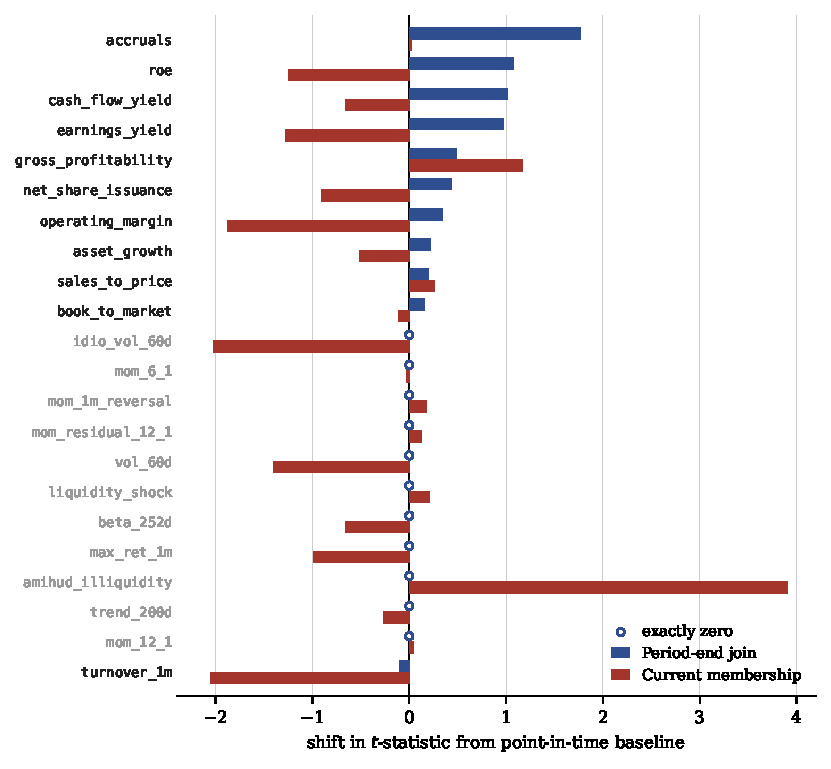
\includegraphics[width=0.86\textwidth]{figures/fingerprints.pdf}
\caption{Shift in $t$-statistic from the point-in-time baseline, all twenty-two factors,
ordered by dating shift. Factor names in dark type read a filed fundamental; those in
grey use only price and volume. The eleven price-only factors carry an open marker rather than a bar on the
period-end series: their shift is exactly zero, to machine precision. The survivorship series has no
zeros anywhere, and its largest movement, \fac{amihud\_illiquidity} at $+3.91$, belongs
to a factor that dating bias cannot touch.}
\label{fig:fingerprints}
\end{figure}

The distortions do not overlap. Figure~\ref{fig:fingerprints} shows both shift vectors on
a common axis, and Table~\ref{tab:families} summarises them by factor family.

\begin{table}[h]
\centering
\small
\begin{tabular}{lll}
\toprule
Factor family & Period-end join & Current membership \\
\midrule
Price and volume & \textbf{Untouched, exactly} & Heavily distorted \\
Value and quality & Inflated; 4 false positives & Mixed, mostly weakened \\
Liquidity and volatility & Untouched & Sign flips, false positives \\
Direction of effect & Uniform inflation & Relocation, not inflation \\
\bottomrule
\end{tabular}
\caption{The two distortions by factor family.}
\label{tab:families}
\end{table}

Quantitatively, the two shift vectors across the twenty-two factors correlate at
$-0.088$. They are not two versions of ``results look better''; they are close to
independent directions in factor space. They also disagree in sign on value: dating
inflates \fac{earnings\_yield} and \fac{roe} by $+0.98$ and $+1.07$ $t$-units,
survivorship deflates them by $-1.28$ and $-1.24$.

One property is a hard constraint rather than a tendency. Under dating bias the eleven
price-only factors are unchanged to machine precision, because they never read a filed
figure. An anomalously strong illiquidity result therefore cannot be produced by dating
bias, whatever else is true of the study.

\subsection{The proposed inversion, and what it would require}
\label{sec:inversion}

This structure suggests reading the implication backwards. A study with a suspiciously
strong illiquidity premium and a dead low-volatility anomaly has a universe problem. A
study whose value and quality factors clear $t = 2$ while its price factors look ordinary
has a dating problem.

Formally, model an observed table of $t$-statistics as
\begin{equation}
t = \tau + \delta_b + \varepsilon,
\end{equation}
where $\tau$ is the study's true factor performance, $\delta_b$ is the signature of bias
$b$ (measured, with $\delta_{\text{none}} = 0$), and $\varepsilon$ is sampling noise.
Since $\tau$ is unknown and twenty-two dimensional, $b$ is not identified without further
structure. Three sources of structure are available, in increasing order of assumption:
exclusion from the exact-zero constraint of Section~\ref{sec:dating}; within-family
contrasts that absorb the unknown level of $\tau$; and projection onto each signature
after removing family means, whose reference distribution under exchangeable $\tau$
yields a $p$-value rather than a label.

We state plainly that this inversion is proposed and not tested. Four conditions would
have to hold, and each is a gate rather than a caveat:

\begin{enumerate}
\item \textbf{Signature stability.} The shift vectors must be properties of the errors,
not of the 2014--2026 sample. This requires re-measurement on disjoint subperiods and
random half-universes.
\item \textbf{Signature uncertainty.} A point estimate cannot support a test. The
sampling covariance of each shift vector must be estimated.
\item \textbf{Separability under realistic noise.} Whether the two errors remain
separable at the noise level of a twelve-year study is an empirical question.
\item \textbf{Calibration before application.} Any output must be a $p$-value or a
posterior with a reference distribution behind it, never a bare label.
\end{enumerate}

Labelled data for the third gate is free: biased panels are generated by the pipeline
itself, so the inversion can be validated at scale without any external dataset or
annotation.

\section{Limitations}
\label{sec:limits}

\begin{itemize}
\item One index, one country, 2010--2026. The fingerprints are measured on the S\&P 500
and should not be assumed to transfer to small caps or non-US markets.
\item Membership spells are reconstructed from a public wiki revision history, not CRSP.
The survivorship arm inherits whatever that approximation gets wrong.
\item Fundamental coverage begins in 2010 because of the XBRL mandate phase-in, so the
dating arm cannot speak to the pre-XBRL era.
\item The two arms are not additively decomposable. The survivorship arm rebuilds forward
returns per universe, because a biased study never observes the returns of the names it
excludes. Real studies contain several errors at once and the signatures may not compose.
\item A study reporting five factors gives a five-dimensional observation, and the
exclusion constraint does not apply at all if none of them are price-only.
\item The inversion in Section~\ref{sec:inversion} is untested. Sections~\ref{sec:dating}
and~\ref{sec:surv} are measurements.
\end{itemize}

\section{Conclusion}

Two common data-handling errors distort a factor study in different and identifiable
ways. The period-end join inflates fundamental factors uniformly by 59\% of true IC and
manufactures four false discoveries while leaving price factors provably untouched.
Current-membership conditioning relocates rather than inflates, flipping illiquidity to
significance and inverting the low-volatility anomaly, through a channel better described
as a forward-looking growth filter than as a survival filter.

Neither distortion is visible in a Sharpe ratio. Both are visible in the cross-section of
what a study reports. Whether that visibility supports reliable inference from a table to
its underlying error is the open question, and Section~\ref{sec:inversion} states what
would have to be established before it could be claimed.

\paragraph{Reproduction.} All results reproduce with \texttt{make bias}. The dating arm is
\texttt{scripts/pit\_vs\_naive.py}; the survivorship arm is
\texttt{scripts/survivorship.py}. Per-factor outputs are written to
\texttt{reports/pit\_vs\_naive.csv} and \texttt{reports/survivorship.csv}. Prices are
fetched per user rather than redistributed. The point-in-time fundamentals layer and the
membership spells are released under CC~BY~4.0.

\begin{thebibliography}{9}
\bibitem{banz1986}
R.~Banz and W.~Breen.
\newblock Sample-dependent results using accounting and market data: some evidence.
\newblock \emph{Journal of Finance}, 41(4):779--793, 1986.
\end{thebibliography}

\end{document}
